% cd ..\..\Users\NikitaSkybytskyi\Desktop\c4s1\nm-mph\lab\lab-2\tex
% cls && pdflatex report.tex && cls && pdflatex report.tex && cls && pdflatex report.tex && start report.pdf
\documentclass[12pt, a4paper]{article}
\usepackage[T2A]{fontenc}
\usepackage[utf8]{inputenc}
\usepackage[english,ukrainian]{babel}
\usepackage{amsmath, amssymb}
\usepackage{verbatim}
\usepackage{minted}
\usepackage{euler}

\usepackage[top = 1.5 cm, left = .75 cm, right = .75 cm, bottom = 1.5 cm]{geometry}
\usepackage[unicode = true, colorlinks = true, linktoc = all, linkcolor = blue]{hyperref}
\usepackage{subcaption}

\usepackage{float}
\usepackage{graphicx}

\usepackage{amsthm}
\newtheorem{lemma}{Лема}
\newtheorem*{lemma*}{Лема}
\newtheorem{theorem}{Теорема}
\newtheorem*{theorem*}{Теорема}
\newtheorem{definition}{Визначення}
\newtheorem*{definition*}{Визначення}
\theoremstyle{definition}
\newtheorem{remark}{Зауваження}
\newtheorem*{remark*}{Зауваження}
\newtheorem{example}{Приклад}
\newtheorem*{example*}{Приклад}
\newtheorem{problem}{Задача}
\newtheorem*{problem*}{Задача}
\newtheorem{solution}{Розв'язок}
\newtheorem*{solution*}{Розв'язок}
\newtheorem{corollary}{Наслідок}
\newtheorem*{corollary*}{Наслідок}

\newcommand{\NN}{\mathbb{N}}
\newcommand{\RR}{\mathbb{R}}
\newcommand{\CC}{\mathbb{C}}
\newcommand{\HH}{\mathcal{H}}
\newcommand{\Max}{\displaystyle\max\limits}
\newcommand{\Sup}{\displaystyle\sup\limits}
\newcommand{\Sum}{\displaystyle\sum\limits}
\newcommand{\Prod}{\displaystyle\prod\limits}
\newcommand{\Int}{\displaystyle\int\limits}
\newcommand{\Iint}{\displaystyle\iint\limits}
\newcommand{\Lim}{\displaystyle\lim\limits}

\newcommand*\diff{\mathop{}\!\mathrm{d}}

\newcommand{\degrees}{^\circ}

\renewcommand{\bf}[1]{\textbf{#1}}
\renewcommand{\epsilon}{\varepsilon}
\renewcommand{\phi}{\varphi}

\newcommand{\ol}[1]{\overline{#1}}
\newcommand{\ul}[1]{\underline{#1}}

\DeclareMathOperator{\signum}{sign}
\DeclareMathOperator{\diam}{diam}
\DeclareMathOperator{\rang}{rang}
\DeclareMathOperator{\const}{const}
\DeclareMathOperator{\cond}{cond}
\DeclareMathOperator{\diagonal}{diag}

\DeclareMathOperator*{\Min}{min}

\setlength\parindent{0pt}
\allowdisplaybreaks

\newcommand{\cover}[2]{
\begin{center}
\hfill \break
  М{\footnotesizeІНІСТЕРСТВО ОСВІТИ ТА НАУКИ} У{\footnotesizeКРАЇНИ} \\
  К{\footnotesizeИЇВСЬКИЙ НАЦІОНАЛЬНИЙ УНІВЕРСИТЕТ ІМЕНІ} Т{\footnotesizeАРАСА} Ш{\footnotesizeЕВЧЕНКА} \\ 
  Ф{\footnotesizeАКУЛЬТЕТ КОМП'ЮТЕРНИХ НАУК ТА КІБЕРНЕТИКИ} \\
  К{\footnotesizeАФЕДРА ОБЧИСЛЮВАЛЬНОЇ МАТЕМАТИКИ}
\end{center}

\vfill 

\begin{center}
  \large{
    Звіт до лабораторної роботи №{#1} на тему: \\ 
    \guillemotleft{}{#2}\guillemotright{}
  }
\end{center}

\vfill 

\begin{flushright}
  Виконав студент групи ОМ-4 \\
  Скибицький Нікіта
\end{flushright}

\vfill 

\begin{center}
    Київ, 2019
\end{center}

\thispagestyle{empty} 
\newpage
}

\newenvironment{system}{%
  \begin{equation}%
    \left\{%
      \begin{aligned}%
}{%
      \end{aligned}%
    \right.%
  \end{equation}%
}
\newenvironment{system*}{%
  \begin{equation*}%
    \left\{%
      \begin{aligned}%
}{%
      \end{aligned}%
    \right.%
  \end{equation*}%
}

\newcommand{\pluseqq}{{\:\:+\!\!=\:\:}}


\begin{document}

\cover{2}{Чисельне розв'язування крайових задач математичної фізики. \\ Метод скінченних елементів}

\tableofcontents

\numberwithin{equation}{section}
\section{Постановка задачі}

\subsection{Загальна постановка задачі}

Знайти наближений розв'язок наступної задачі проекційним та варіаційним методами: задано рівняння
\begin{equation}
    \label{eq:1.1}
    - \frac{\diff}{\diff x} \left( k(x) \cdot \frac{\diff u(x)}{\diff x} \right) + q(x) \cdot u(x) = f(x), \quad a < x < b,
\end{equation}
з крайовими умовами
\begin{align}
    \label{eq:1.2}
    -k(x) \cdot \frac{\diff u(x)}{\diff x} + \alpha_1 u(x) &= \mu_1, \quad x = a, \\
    \label{eq:1.3}
    k(x) \cdot \frac{\diff u(x)}{\diff x} + \alpha_2 u(x) &= \mu_2, \quad x = b,
\end{align}
де
\begin{align}
    \label{eq:1.4}
    k(x) &= k_1 \sin(k_2 x) + k_3, \\
    & \quad k(x) > 0, \nonumber \\
    \label{eq:1.6}
    q(x) &= q_1 \sin(q_2 x) + q_3, \\
    & \quad q(x) \ge 0, \nonumber \\
    & \quad \alpha_1, \alpha_2 > 0. \nonumber
\end{align}

\subsubsection{Зауваження}

Задача \emph{модельна}, тому функцію $f(x)$ і константи $\mu_1$, $\mu_2$ виражаємо з відповідних рівностей:
\begin{align}
    \label{eq:1.7}
    f(x) &= -(k(x) \cdot u'(x))' + q(x) \cdot u(x), \\
    \label{eq:1.8}
    \mu_1 &= -k(a) \cdot u'(a) + \alpha_1 u(a), \\
    \label{eq:1.9}
    \mu_2 &= k(b) \cdot u'(b) + \alpha_2 u(b),
\end{align}
де $u(x)$ --- точний розв'язок задачі, функція $u(x) = m_1 \sin(m_2 x) + m_3$.

\subsection{Параметри варіанту}

\begin{table}[H]
    \centering
    \begin{tabular}{|c|c||c|c||c|c|c||c|c|c||c|c|c|}
        \hline
        $a$ & $b$ & $\alpha_1$ & $\alpha_2$ & $k_1$ & $k_2$ & $k_3$ & $q_1$ & $q_2$ & $q_3$ & $m_1$ & $m_2$ & $m_3$ \\ \hline
        0 & 4 & 4 & 2 & 2 & 3 & 1 & 0 & 2 & 3 & 2 & 2 & 1 \\ \hline
    \end{tabular}
\end{table}

\section{Теоритичні відомості}

\setcounter{subsection}{-1}
\subsection{Аналітичні маніпуляції}

Перш за все, виразимо функцію $f(x)$ і константи $\mu_1$, $\mu_2$ з рівностей \eqref{eq:1.7}--\eqref{eq:1.9}:
\begin{align}
    \label{eq:2.0.1}
    f(x) &= 10 \sin(2 x) + 2 \sin(3 x) - 2 \cos(x) - 22 \cos(5x) + 1, \\
    \label{eq:2.0.2}
    \mu_1 &= 0, \\
    \label{eq:2.0.3}
    \mu_2 &= 6.
\end{align}

\numberwithin{equation}{subsection}
\subsection{Алгоритм}

Нехай задане рівняння 
\begin{equation}
    \label{eq:2.1.1}
    A u = f,
\end{equation}
де $A: \HH \rightarrow \HH$ ($\HH$ --- гільбертовий простір), та неоднорідні крайові умови виду \eqref{eq:1.2}--\eqref{eq:1.3}. Наближення розв'язку $u_n(x)$ задачі \eqref{eq:2.1.1} будемо шукати у скінченновимірному підпросторі $\HH_n$, базис якого утворений лінійно незалежною координатною системою функцій $\{\phi_i\}_{i = 0}^n$, тобто у вигляді
\begin{equation}
    \label{eq:2.1.2}
    u_n(x) = \Sum_{i = 1}^n y_i \phi_i(x).
\end{equation}

Одразу зауважимо, що тоді $u(x_i) = y_i$.

\subsubsection{Координатна система функцій}

Систему функцій $\{\phi_i\}_{i = 0}^n$ побудуємо наступним чином: на інтервалі $[a, b]$ побудуємо рівномірну сітку з $(n + 1)$-го вузла:
\begin{equation}
    \label{eq:2.1.3}
    x_i = \frac{(n - i) a + i b}{n}, \quad i = \overline{0..n}.
\end{equation}

\begin{minipage}[t]{.475\textwidth}
    \begin{example*}
    $\{\phi_i\}_{i = 1}^{n - 1}$ --- так звані штафетини:
        \begin{equation}
        \label{eq:2.1.4}
            \phi_i(x) = \begin{cases}
                \frac{x - x_{i - 1}}{h_i}, & x_{i - 1} \le x \le x_i, \\[.5ex]
                \frac{x_{i + 1} - x}{h_i}, & x_i \le x \le x_{i + 1}, \\
                0, & \text{інакше}.
            \end{cases}
        \end{equation}
        А також $\phi_0, \phi_n$ --- напівштафетини, у яких обрізані половини, які виходять за $[x_0, x_n]$,
        \begin{align}
            \phi_0(x) &= \begin{cases}
                \frac{x_1 - x}{h_i}, & x_0 \le x \le x_1, \\
                0, & \text{інакше}.
            \end{cases} \\
            \phi_n(x) &= \begin{cases}
                \frac{x - x_{n - 1}}{h_i}, & x_{n - 1} \le x \le x_n, \\
                0, & \text{інакше}.
            \end{cases}
        \end{align}
    \end{example*}
\end{minipage}
\begin{minipage}[t]{.05\textwidth}
    $\left.\right.$
\end{minipage}
\begin{minipage}[t]{.475\textwidth}
    Графіки цих функцій мають вигляд
    \begin{figure}[H]
        \centering
        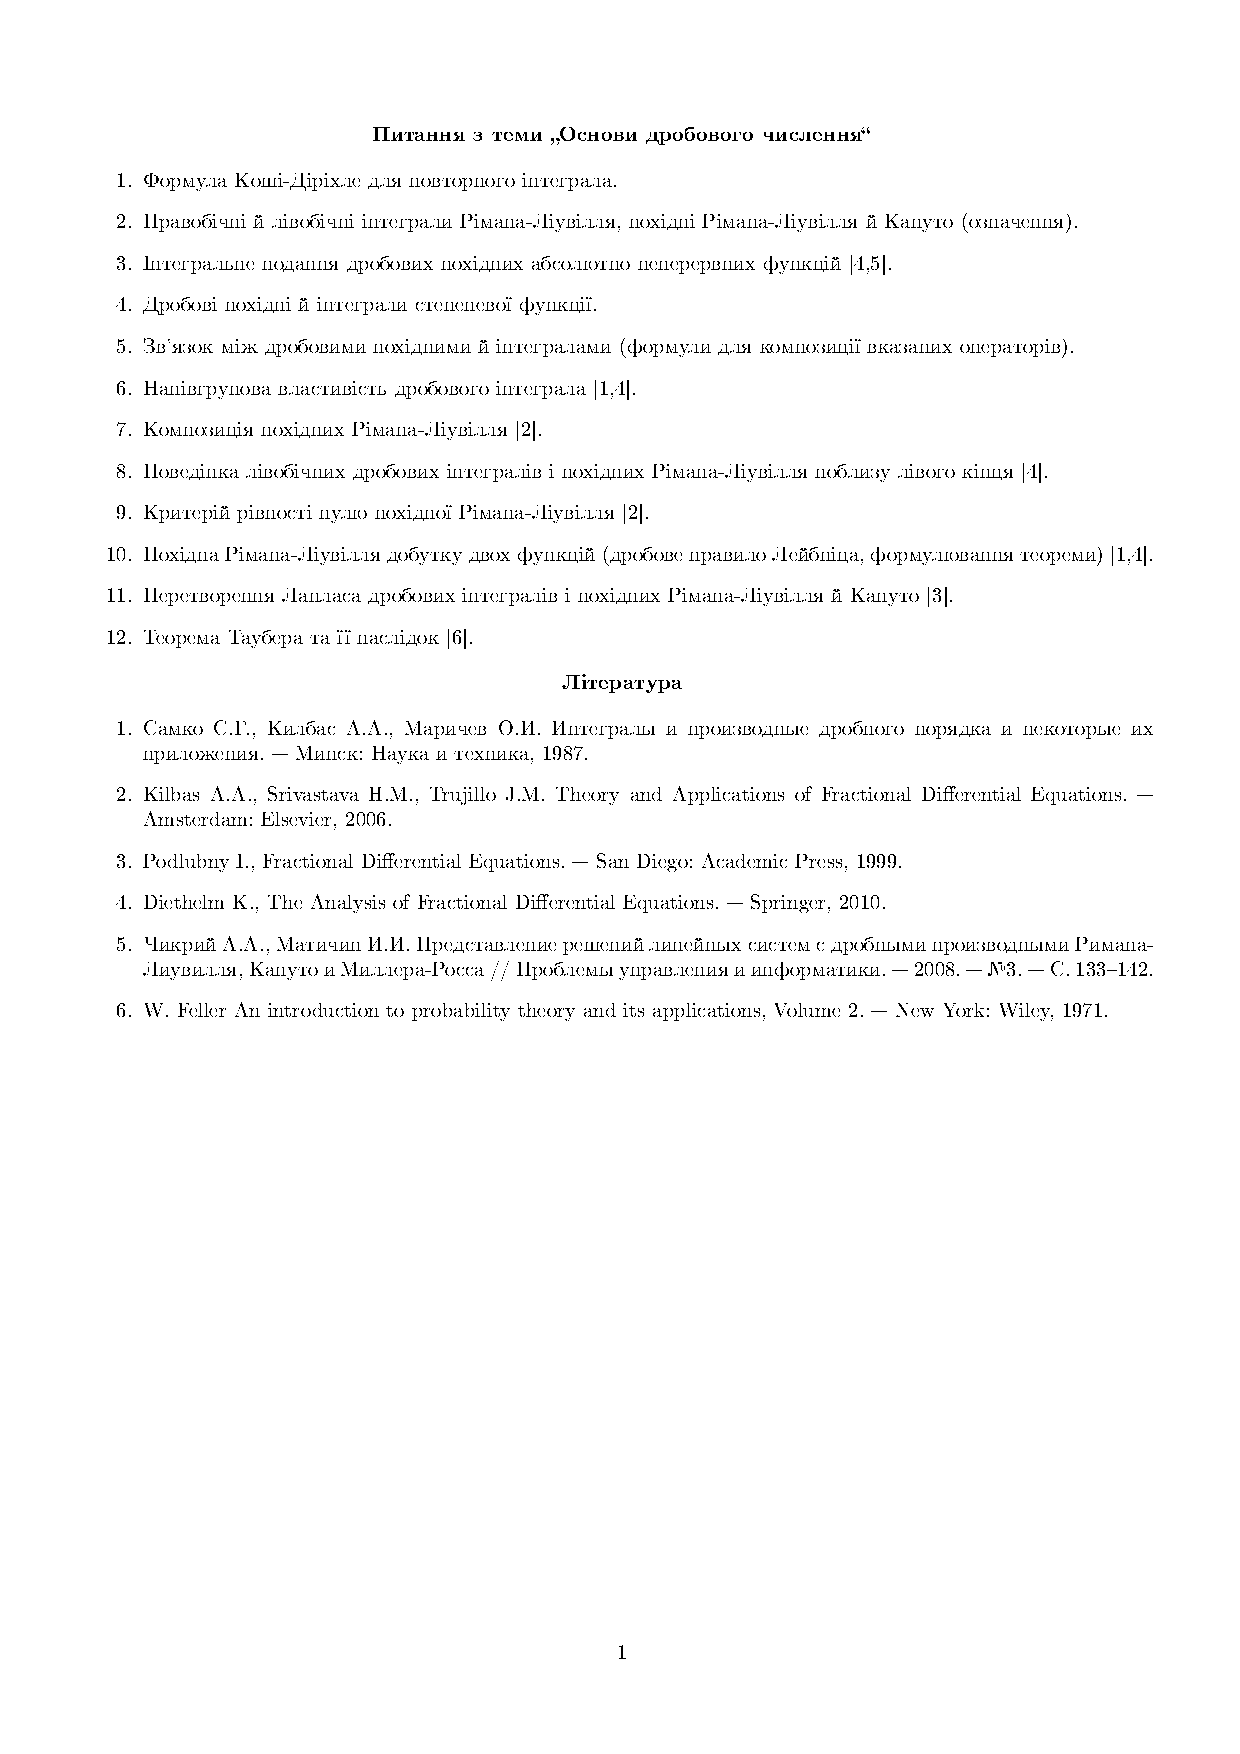
\includegraphics[width=.789473684\textwidth]{1.mps} % .375 of entire textwidth
        \caption{``штафетина'' від $x_{i - 1}$ до $x_{i + 1}$.}
    \end{figure}
\end{minipage} \medskip

\textit{Зауваження:} у коді зручно задавати їх у вигляді \texttt{phi[i](x) := max(0, 1 - abs(x - x[i]) / h) * (a <= x <= b)}, або навіть без індикатора належності $x$ області $[a, b]$ якщо це гарантує клієнтський код. \medskip

\subsection{Виведення системи}

Розв'язок шукаємо як мінімум функціонала
\begin{equation}
    \label{eq:2.1.5}
    \Phi_n = \Min_{u_n \in \HH_n} \Phi (u_n) = \Min_{u_n \in \HH_n} \left\| A u_n - f \right\|^2 
\end{equation}

Відомо (з леми), що $G(u_n, \phi_i) = \ell(\phi_i)$, при $i = \overline{0..n}$. Це рівносильно системі:
\begin{equation}
    \label{eq:2.1.6}
    \Sum_{i = 1}^n c_i G(\phi_i, \phi_j) = \ell(\phi_j), \quad j = \overline{0..n},
\end{equation}
або, іншими словами,
\begin{equation}
    \label{eq:2.1.7}
    \Sum_{i = 1}^n a_{i,j} y_i = b_j, \quad j \in \overline{0..n}.
\end{equation}

Він досягається на розв'язку наступної системи $(n+1)$-го алгебраїчного рівняння відносно $y_i$:
\begin{equation}
    \label{eq:2.1.8}
    \Sum_{i = 1}^n c_i G(\phi_i, \phi_j) = \ell(\phi_j), \quad j = \overline{0..n},
\end{equation}
де
\begin{equation}
    \label{eq:2.1.9}
    \begin{aligned}
        a_{ij} &= G(\phi_i, \phi_j) = \Int_a^b (-k(x) \phi_i'(x))' \phi_j(x) + q(x) \phi_i(x) \phi_j(x) \diff x = \\
        &= \Int_a^b -k(x) \phi_i'(x) \phi_j'(x) + q(x) \phi_i(x) \phi_j(x)  \diff x - \left. k(x) \phi_i'(x) \phi_j(x) \right|_a^b = \\
        &= \Int_a^b -k(x) \phi_i'(x) \phi_j'(x) + q(x) \phi_i(x) \phi_j(x) \diff x + \alpha_1 \phi_i(a) \phi_j(a) %- \mu_1 
        + \alpha_2 \phi_i(b) \phi_j(b) %- \mu_2
        ,
    \end{aligned}
\end{equation}
і
\begin{equation}
    \label{eq:2.1.10}
    b_j = \ell(\phi_j) = \Int_a^b f(x) \phi_j(x) dx + \mu_1 \phi_j(a) + \mu_2 \phi_j(b).
\end{equation}

Зауважимо, що
\begin{equation}
    \phi_i'(x) = \begin{cases}
        \frac{1}{h}, & x_{i - 1} \le x \le x_i, \\
        -\frac{1}{h}, & x_i \le x \le x_{i + 1}, \\
        0, & \text{інакше}.
    \end{cases}
\end{equation}
при $i = \overline{1..n-1}$, і
\begin{equation}
    \phi_0'(x) = \begin{cases}
        -\frac{1}{h}, & x_0 \le x \le x_{1}, \\
        0, & \text{інакше}.
    \end{cases}
    \qquad
    \phi_n'(x) = \begin{cases}
        \frac{1}{h}, & x_{n - 1} \le x \le x_n, \\
        0, & \text{інакше}.
    \end{cases}
\end{equation}

Підставимо точні значення функції $\phi_i(x)$ та їх похідних в систему, матимемо:
\begin{align}
    a_{0, 0} &= \Int_{x_0}^{x_1} \frac{k(x)}{h^2} + q(x) \phi^2_0(x) \diff x + \alpha_1 \phi^2_0(a), \\
    a_{i, i} &= \Int_{x_{i - 1}}^{x_{i + 1}} \frac{k(x)}{h^2} + q(x) \phi^2_i(x) \diff x, \quad i = \overline{1..n-1}, \\
    a_{n, n} &= \Int_{x_{n - 1}}^{x_n} \frac{k(x)}{h^2} + q(x) \phi^2_n(x) \diff x + \alpha_2 \phi^2_n(b), \\
    a_{i, i - 1} &= \Int_{x_{i - 1}}^{x_i} -\frac{k(x)}{h^2} + q(x) \phi_i(x) \phi_{i - 1}(x) \diff x, \quad i = \overline{1..n}, \\
    a_{i, i + 1} &= \Int_{x_i}^{x_{i + 1}} -\frac{k(x)}{h^2} + q(x) \phi_i(x) \phi_{i + 1}(x) \diff x, i = \overline{0..n-1},
\end{align}
а також
\begin{align}
    b_0 &= \Int_{x_0}^{x_1} f(x) \phi_0(x) \diff x + \mu_1, \\
    b_i &= \Int_{x_{i - 1}}^{x_{i + 1}} f(x) \phi_i(x) \diff x, \quad i = \overline{1..n-1}, \\
    b_n &= \Int_{x_{n - 1}}^{x_n} f(x) \phi_n(x) \diff x + \mu_2.
\end{align}

\textit{Зауваження:} $a_{i,j} = 0$ при $|i - j| > 1$, адже тоді області де $\phi_i \ne 0$ та $\phi_j \ne 0$ не перетинаються, і $G(\phi_i, \phi_j) = 0$, отже матриця системи --- тридіагональна і її (систему) можна розв'язувати методом прогонки.

\section{Практична частина}
Було використано мову програмування \verb|python| і бібліотеки \verb|numpy|, \verb|scipy| і \verb|matplotlib|.

\subsection{Похибки}
Відхилення від точного розв'язку в нормі 
\begin{equation}
    \|f\| = \frac{1}{b - a} \int_a^b f^2(x) \diff x:
\end{equation}
\begin{itemize}
    % \item 1 функція: \texttt{2.365293407220804};
    % \item 2 функції: \texttt{1.7687752473908065};
    \item 4 функції: \texttt{0.11072227505224305};
    \item 8 функцій: \texttt{0.059055683092381954};
    \item 16 функцій: \texttt{0.0022117026009372417};
    \item 32 функції: \texttt{0.000455942368470552}.
\end{itemize}

\subsection{Графіки}
% \begin{figure}[H]
%     \begin{subfigure}{.5\textwidth}
%     \centering
%     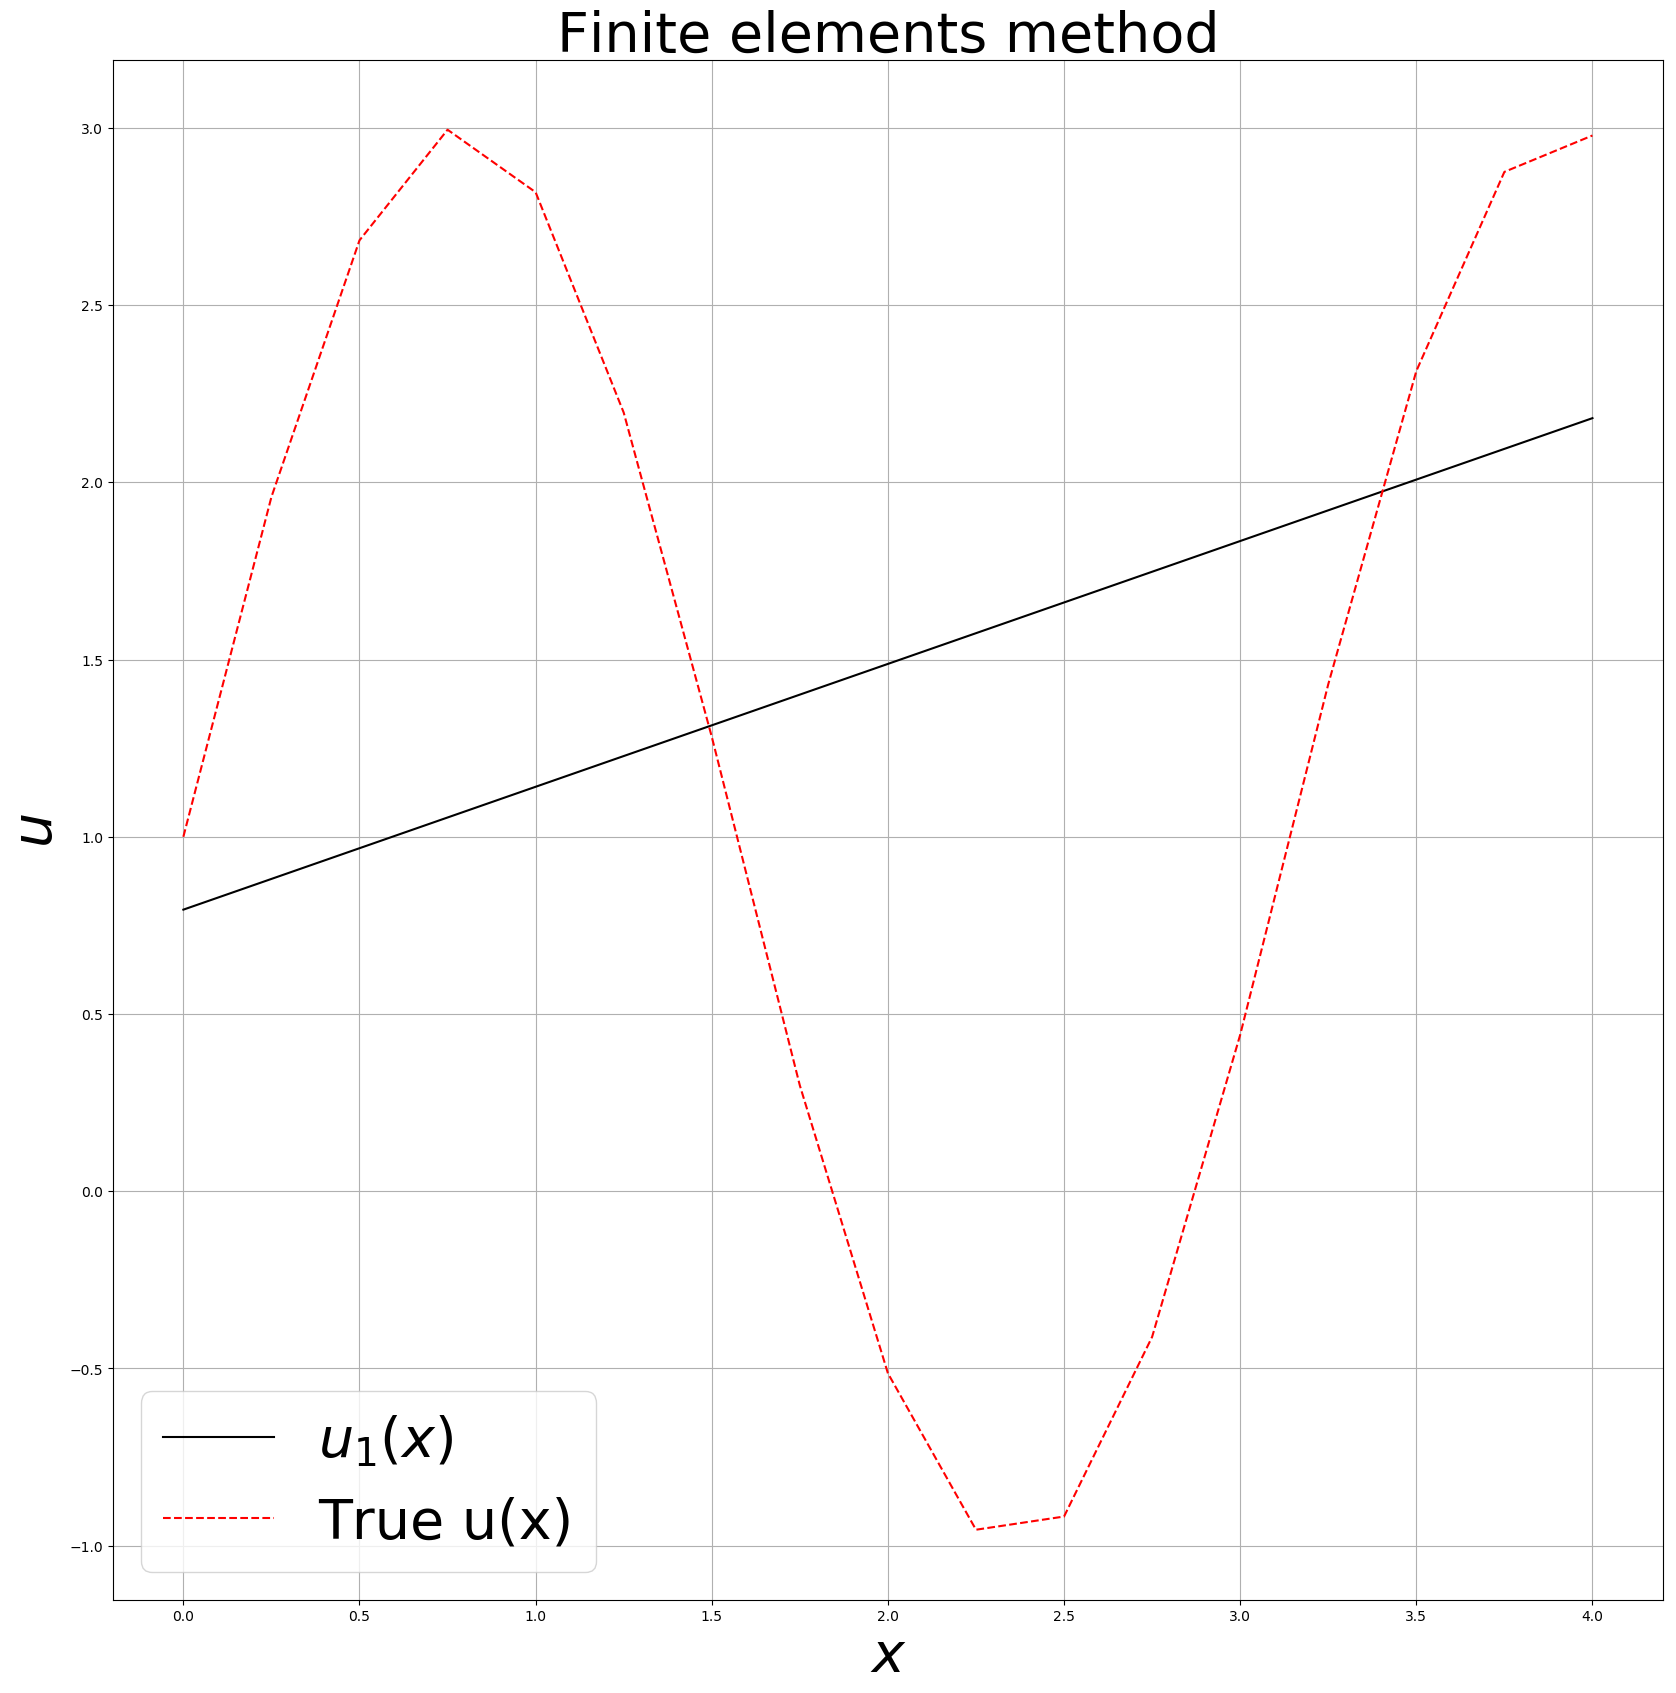
\includegraphics[width=.95\linewidth]{tex/fem_1.png}
%     \caption{1 функція}
%     \end{subfigure}
%     \hfill
%     \begin{subfigure}{.5\textwidth}
%     \centering
%     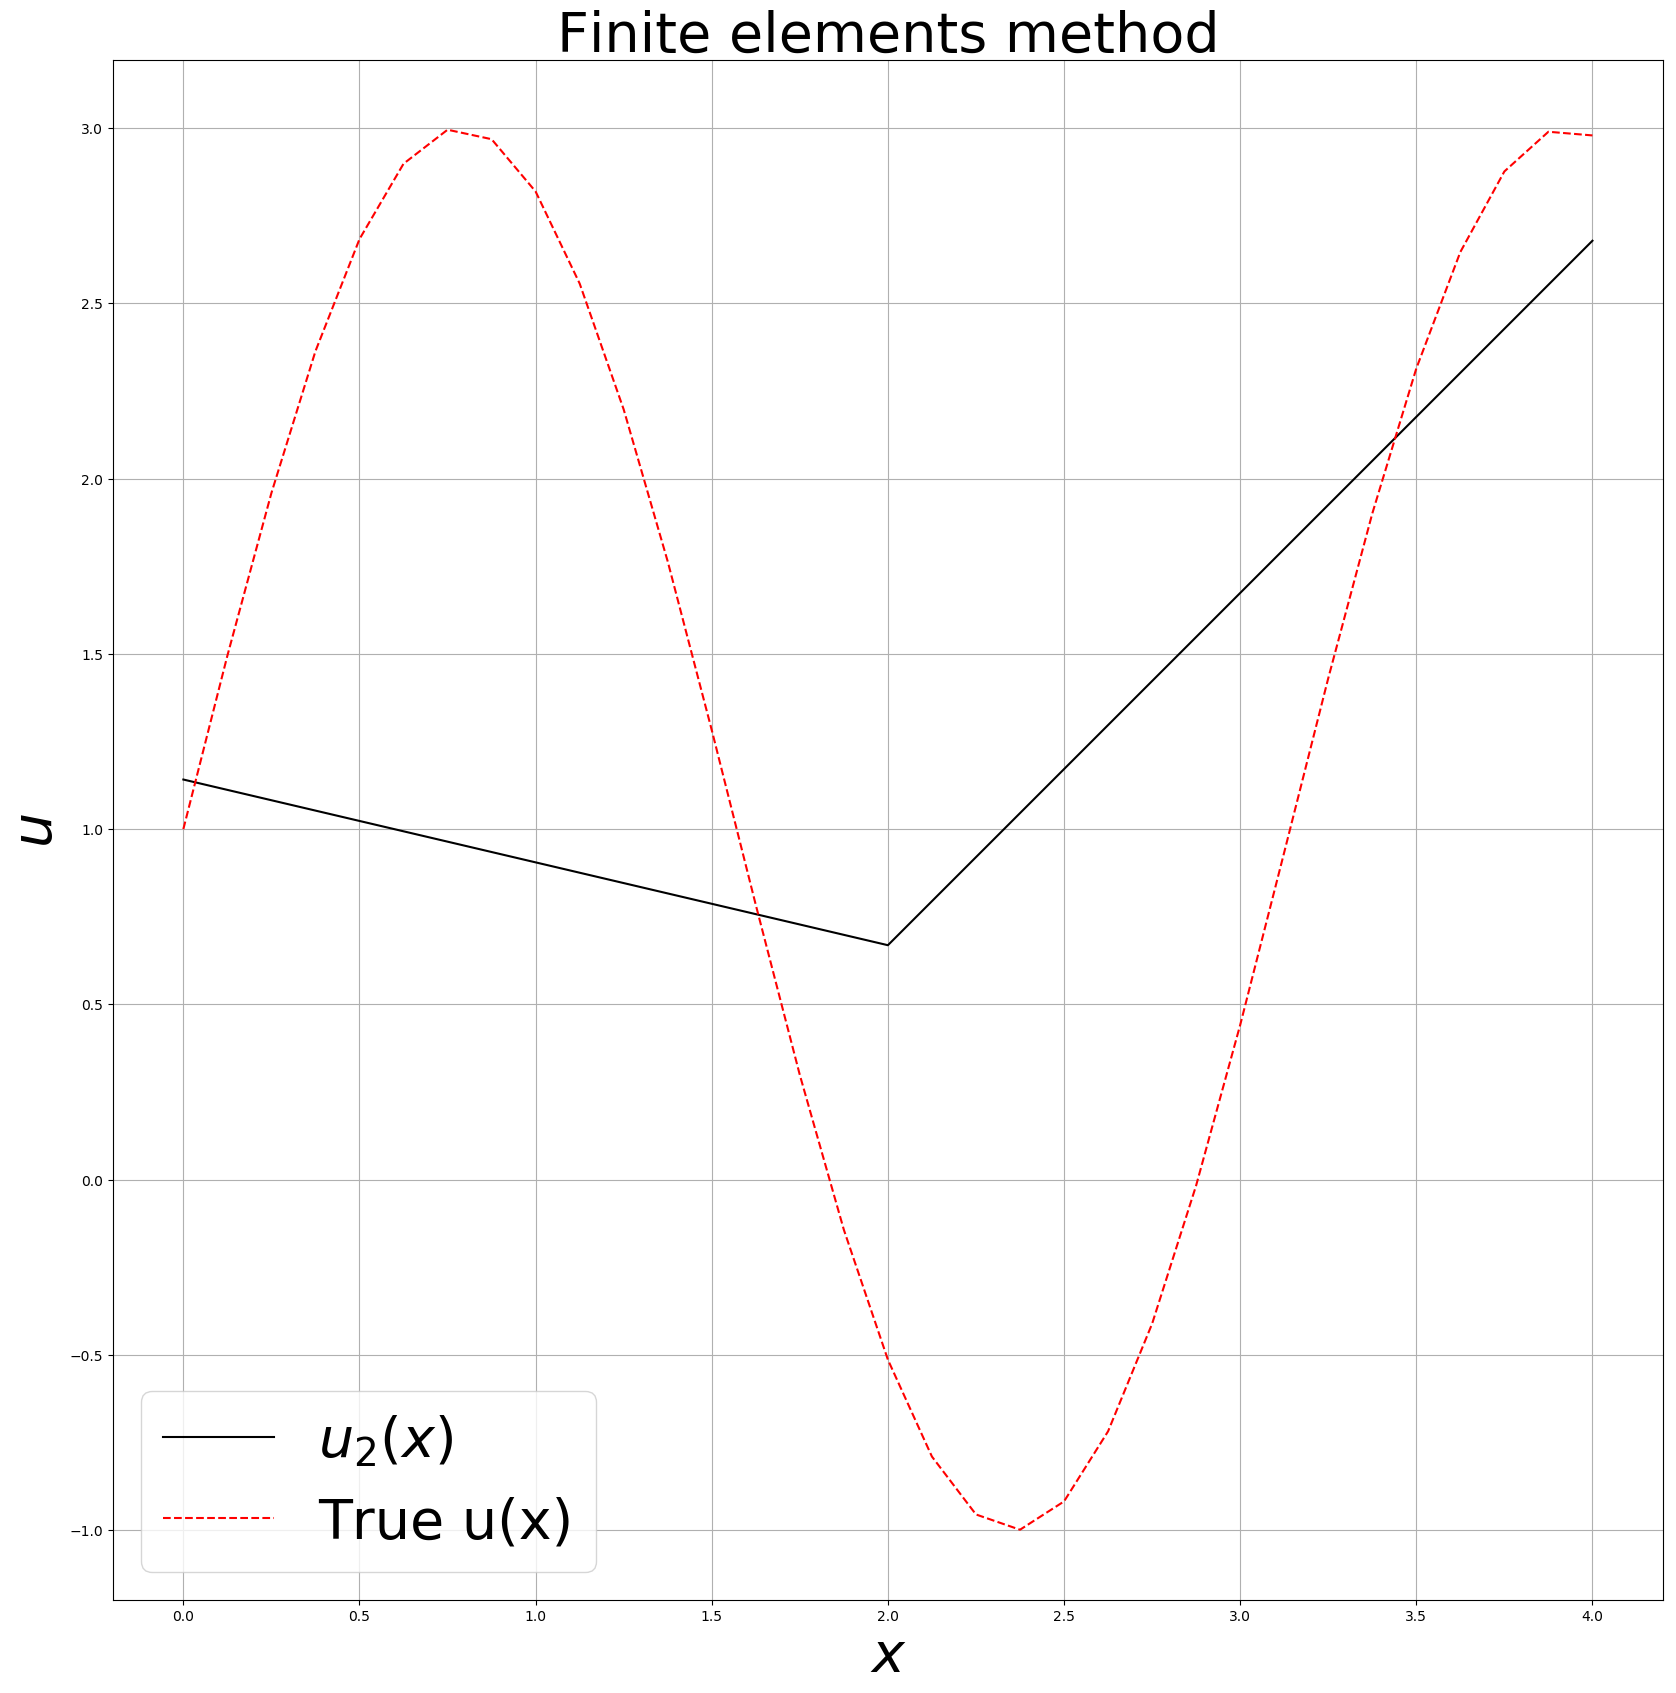
\includegraphics[width=.95\linewidth]{tex/fem_2.png}
%     \caption{2 функції}
%     \end{subfigure}
% \end{figure}

\begin{figure}[H]
    \begin{subfigure}{.5\textwidth}
    \centering
    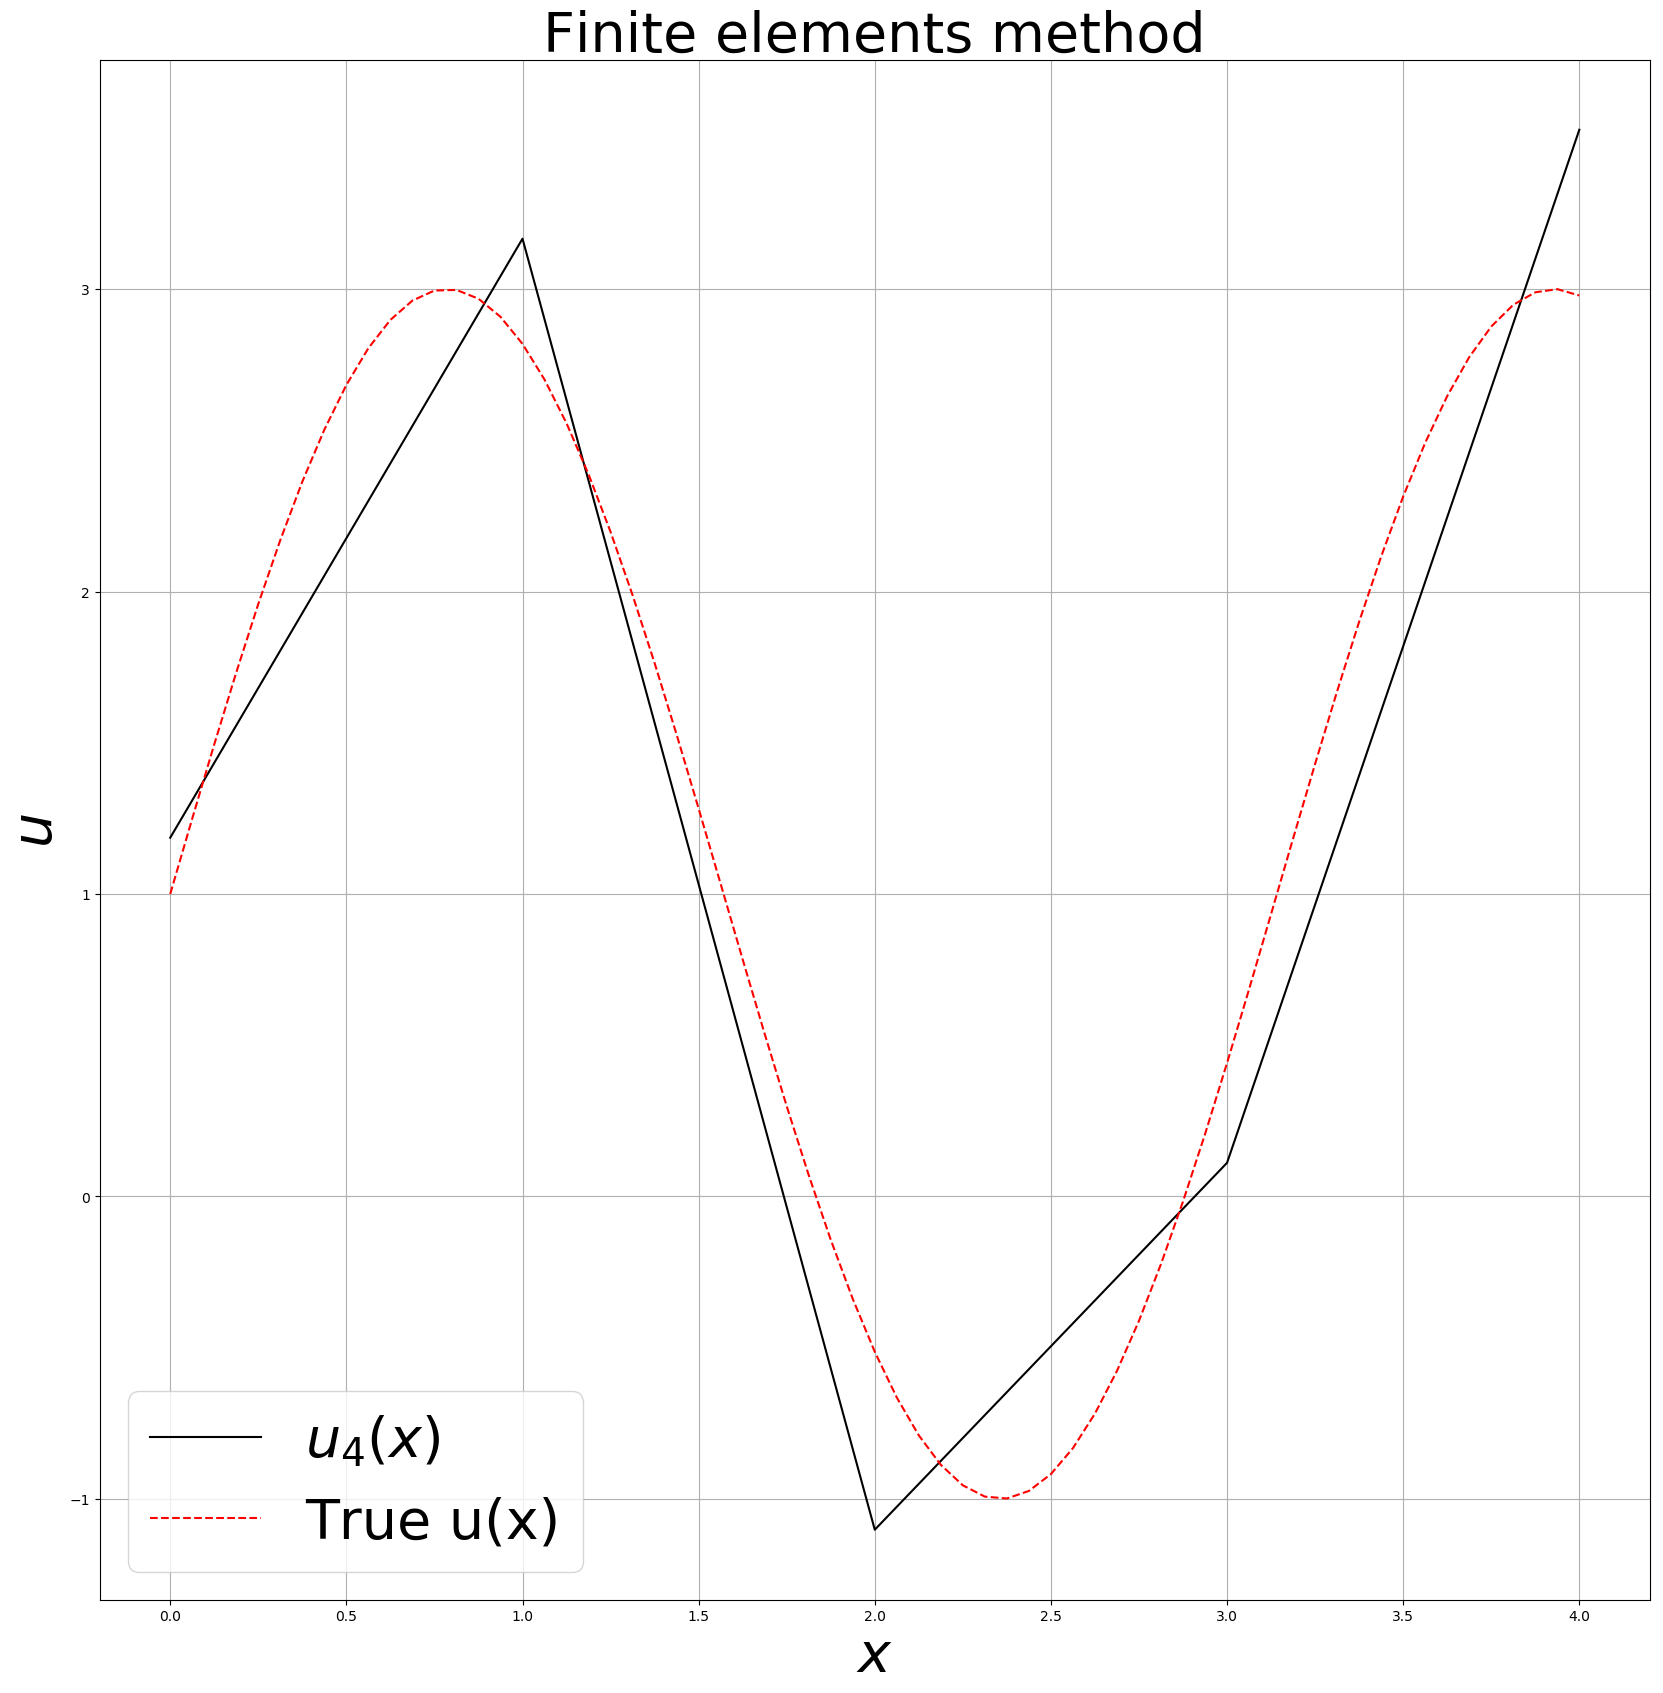
\includegraphics[width=.95\linewidth]{tex/fem_4.png}
    \caption{4 функції}
    \end{subfigure}
    \hfill
    \begin{subfigure}{.5\textwidth}
    \centering
    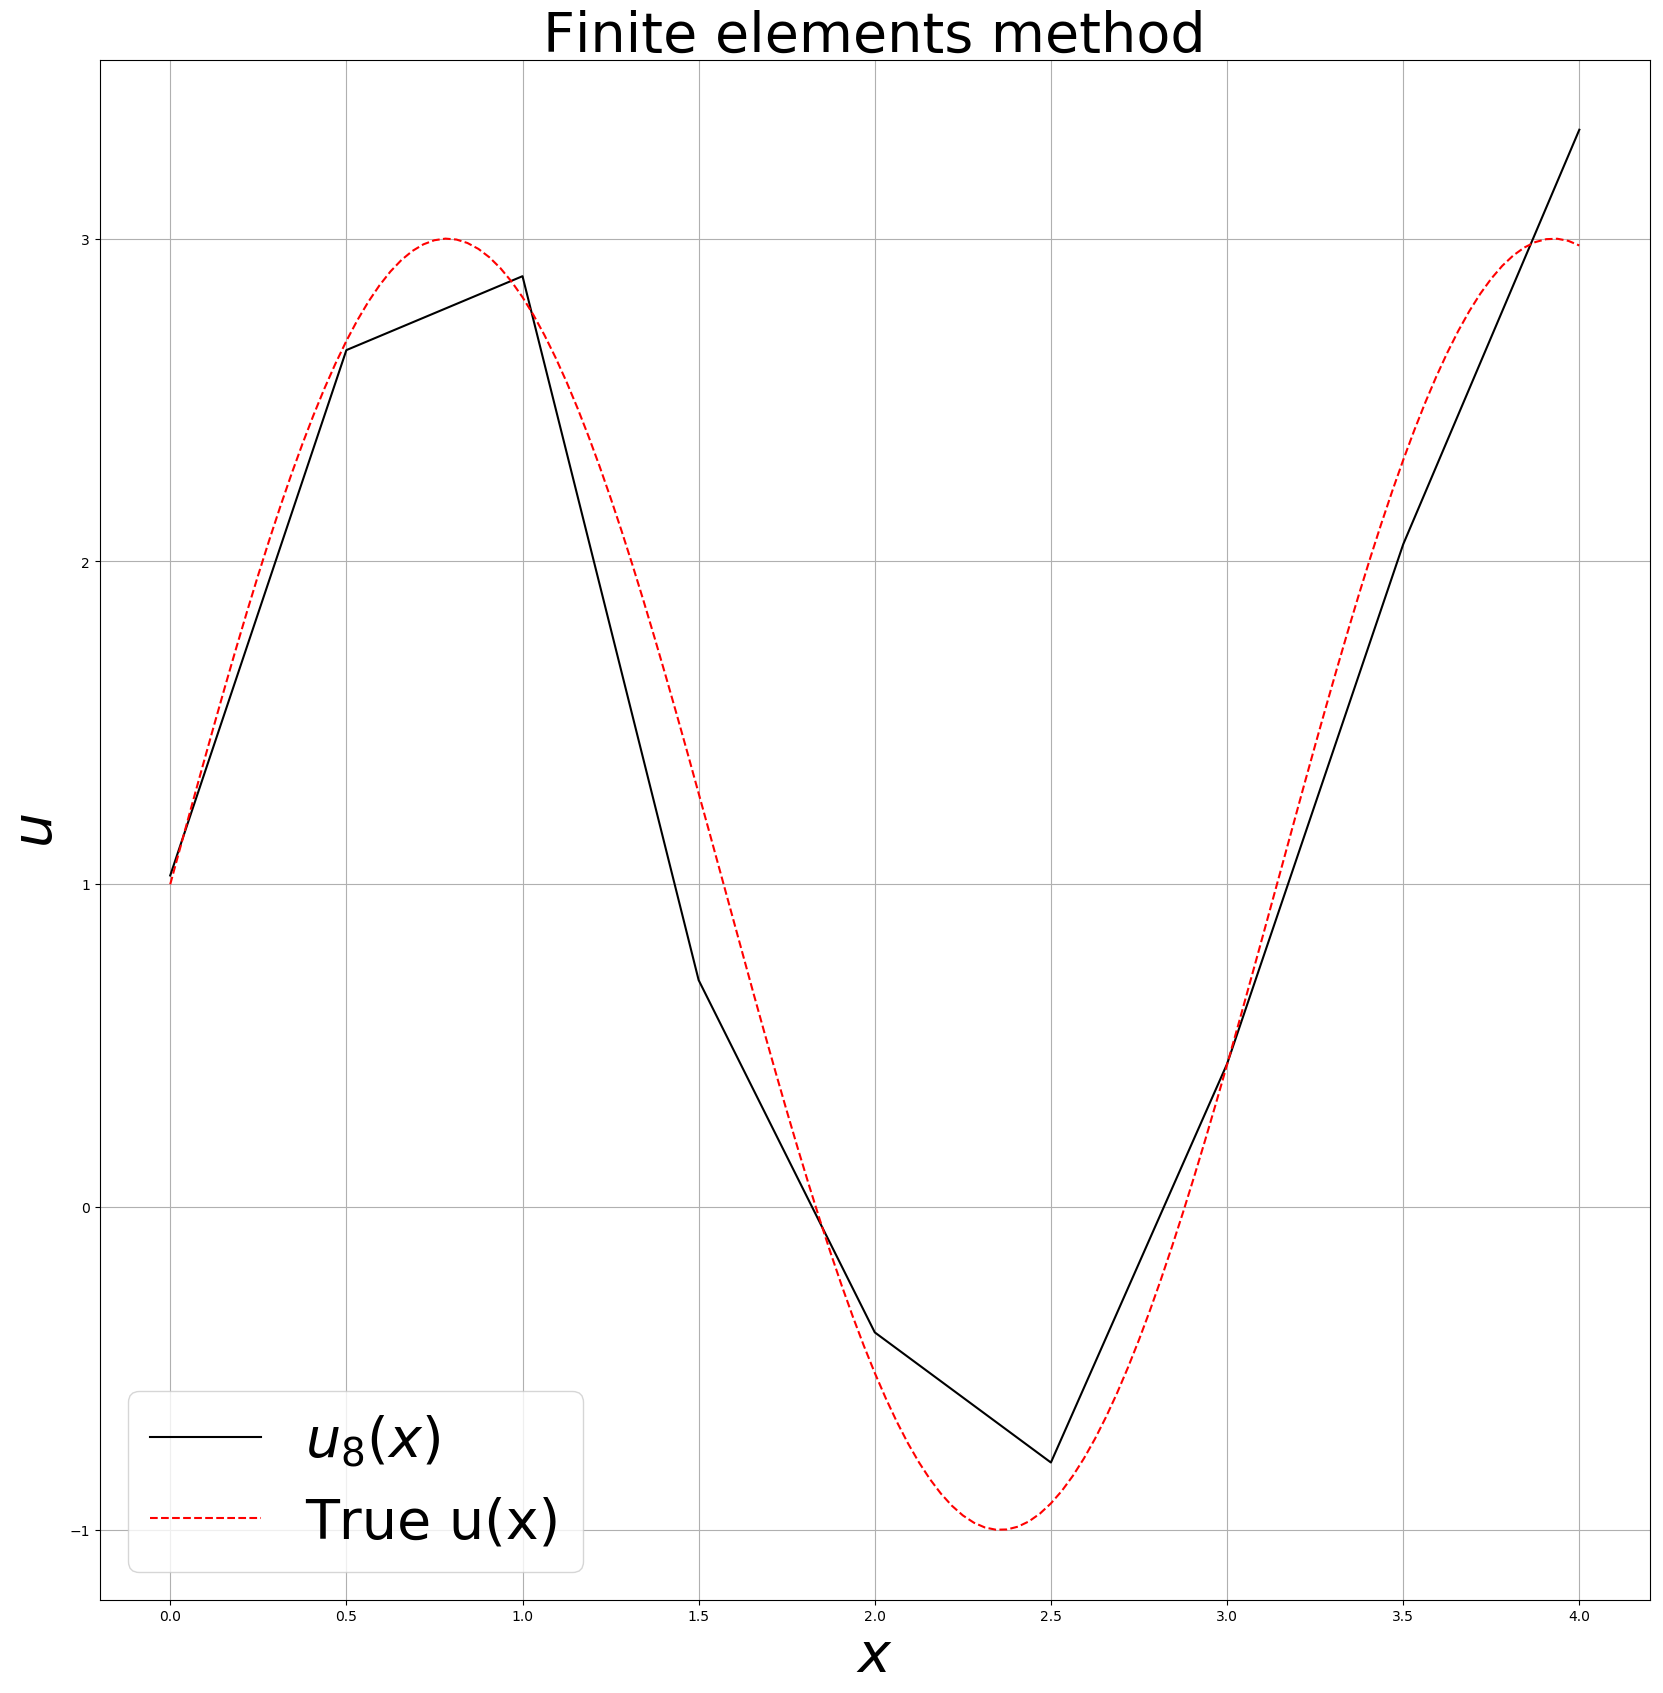
\includegraphics[width=.95\linewidth]{tex/fem_8.png}
    \caption{8 функцій}
    \end{subfigure}
\begin{figure}[H]

\end{figure}[H]
    \begin{subfigure}{.5\textwidth}
    \centering
    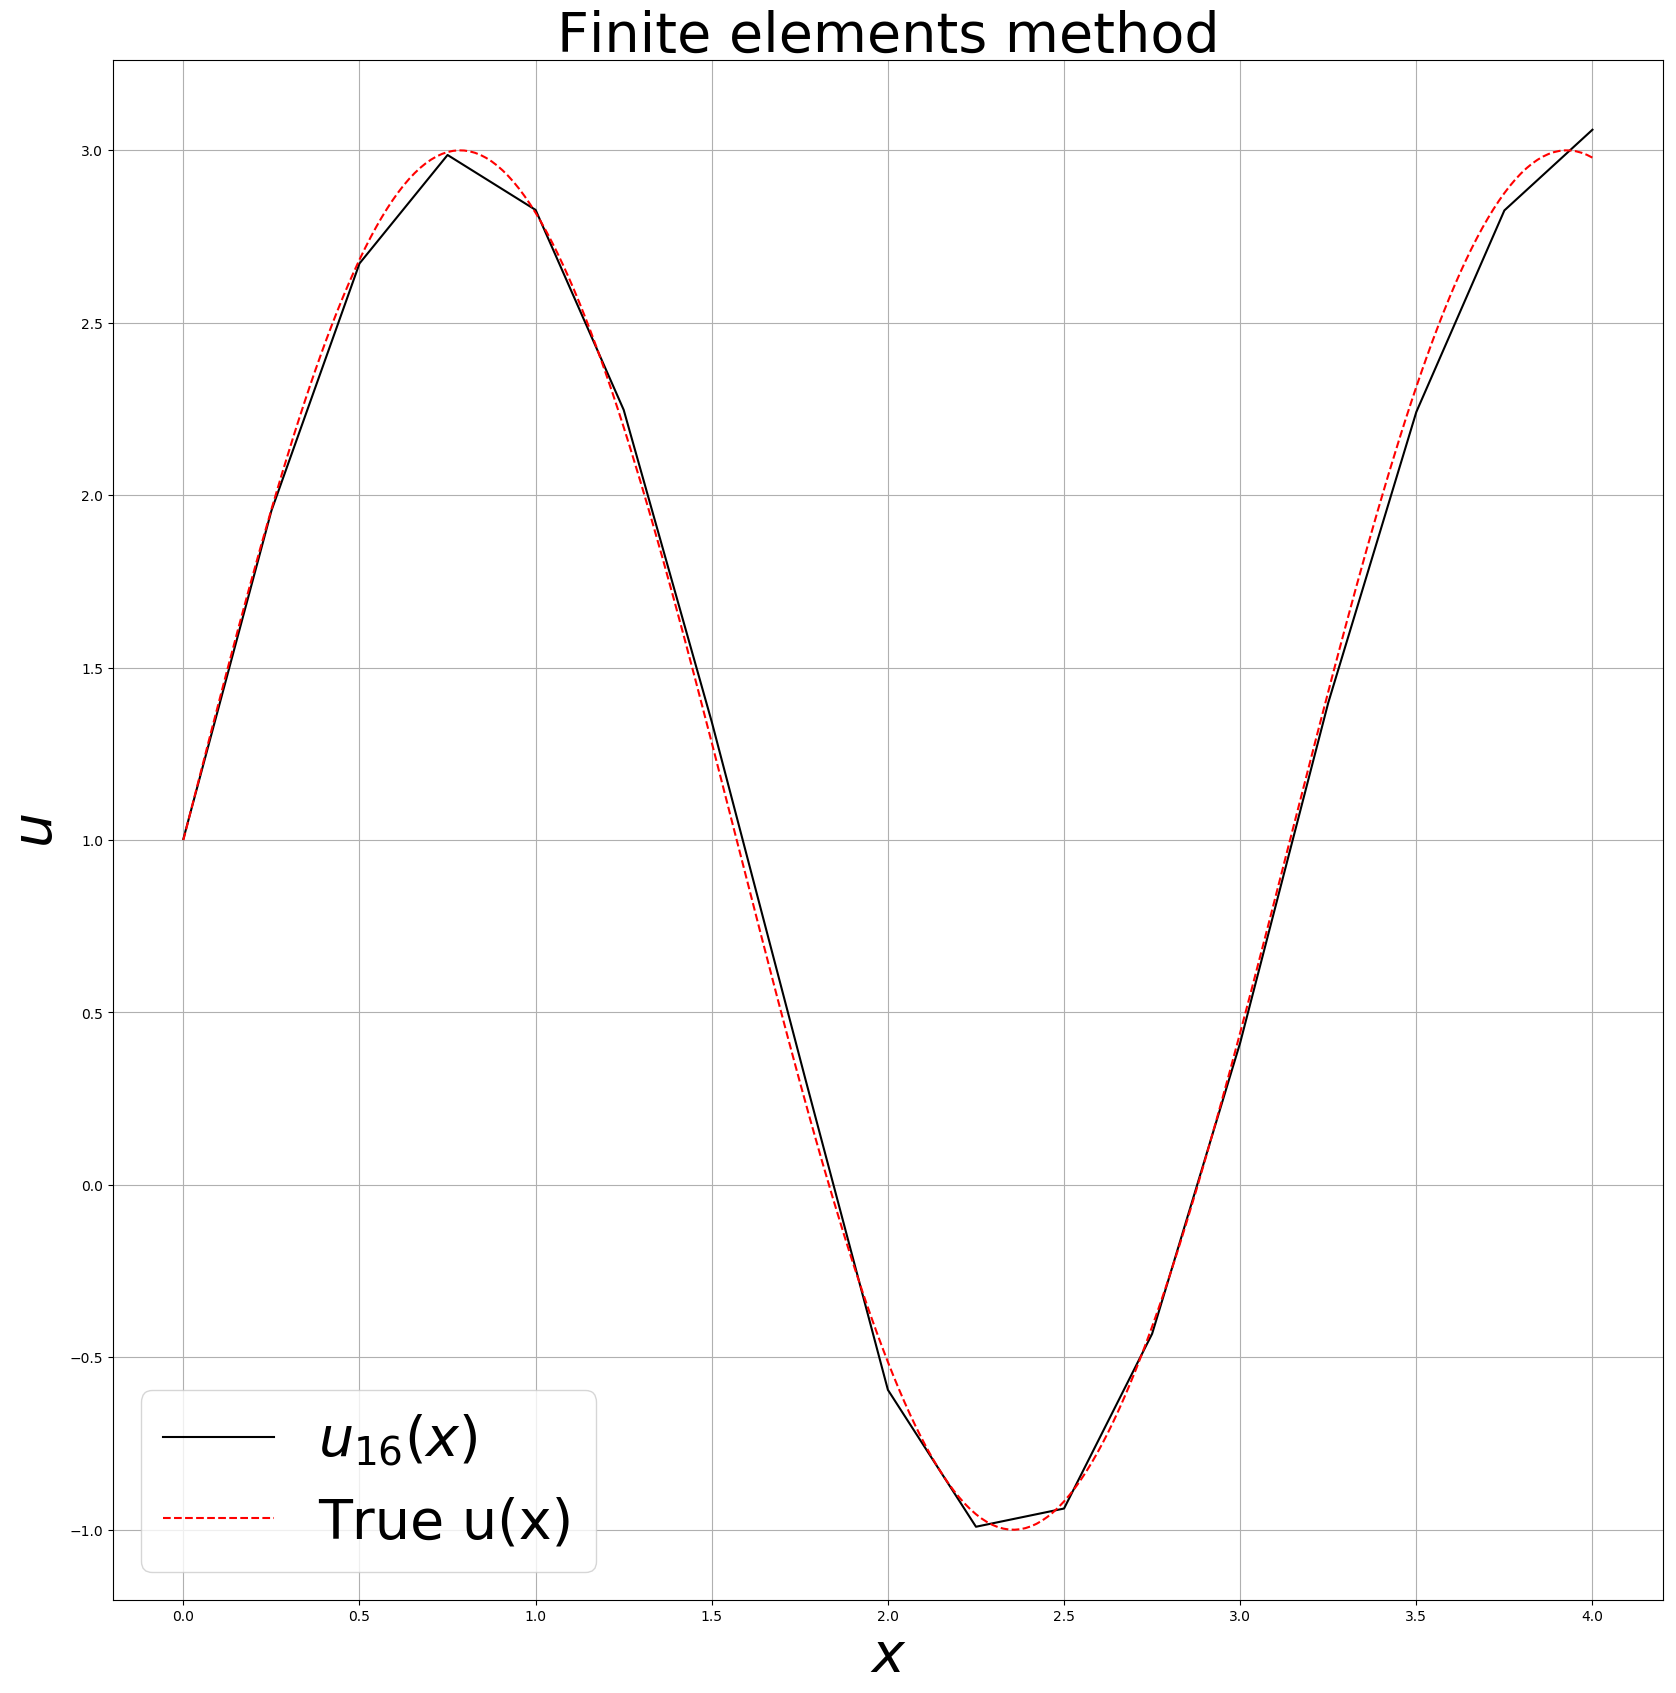
\includegraphics[width=.95\linewidth]{tex/fem_16.png}
    \caption{16 функцій}
    \end{subfigure}
    \hfill
    \begin{subfigure}{.5\textwidth}
    \centering
    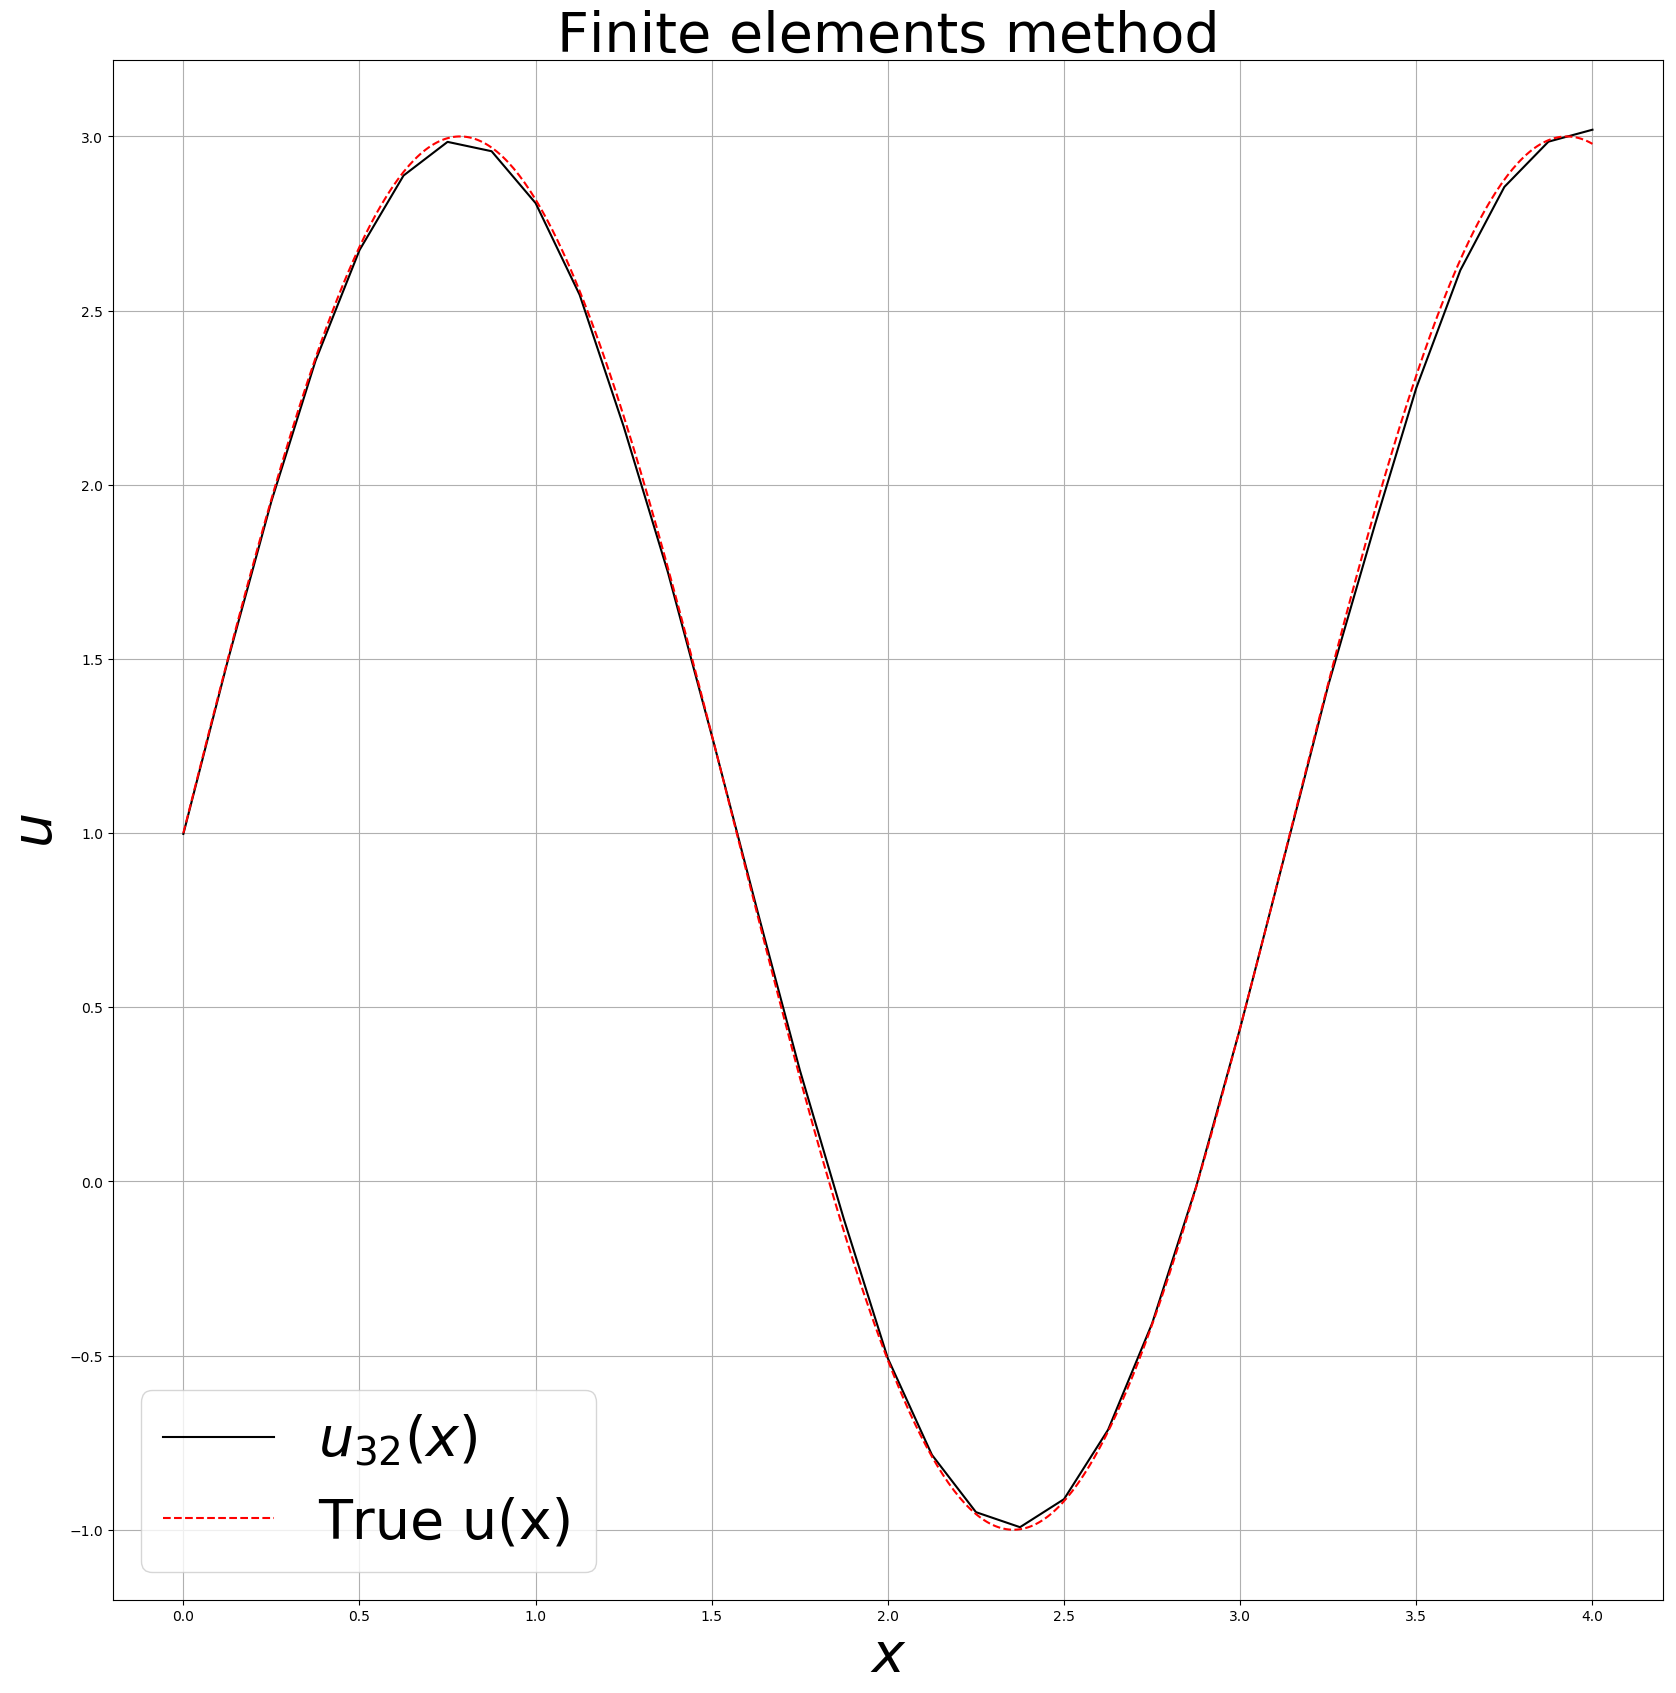
\includegraphics[width=.95\linewidth]{tex/fem_32.png}
    \caption{32 функції}
    \end{subfigure}
\end{figure}

\end{document}
